\chapter{Streams}

\section{Motivation}
There are many data processing applications that deal with streams of relevance-priority data (e.g Sports data, weather data, telemetry (spacecraft, service usage)).
\begin{itemize}
    \item Recent events are valuable, old events are not (and can be discarded or sent to data warehouse after some time)
    \item Users run a static query on an unbounded stream of data
    \item The state of the system must be bounded (limited memory)
    \item Timestamps for events are important (tradeoffs between performance, and accuracy), the order at which events are received is important.
    \item Results can be approximate
\end{itemize}

\section{Push Operators}
Rather than operators pulling in tuples (as in \textit{volcano processing}), operators push tuples to the next stage.
\begin{minted}{cpp}
// templated by the Event data type (for easy testing), would be some vector<variant<int, float, string, ...>>
template<typename Event>
class PushOperator {
public:
    virtual void process(Event data) = 0;
};
\end{minted}
\begin{itemize}
    \item As with volcano and bulk processing we can also send references to data (e.g indexes into a larger backing table) to avoid copies.
    \item Virtual method used to allow operators to be combined into queries at runtime.
    \item Can use \mintinline{cpp}{std::move} to reduce deep copying for large \mintinline{cpp}{Event} types (e.g vectors of variants).
\end{itemize}

\subsection{Naive Implementation}
\subsubsection{Output to Console}
Some form of output operator is required to send data to the user (e.g player positions sent over the network to a live sports match website).
\\
\\ Here a basic Output operator pushes to a stream (e.g a file with \mintinline{cpp}{std::ofstream}, or to the console with \mintinline{cpp}{std::cout}).
\begin{minted}{cpp}
template <typename Event>
class Output : public PushOperator<Event> {
    std::ostream &output_;
public:
    Output(std::ostream &output) : output_(output) {}

    void process(Event data) override { output_ << "->" << data << std::endl; }
};
\end{minted}

\subsubsection{Selection}
\begin{minted}{cpp}
template <typename Event>
class Select : public PushOperator<Event> {
    PushOperator<Event> *plan_;
    std::function<bool(Event &)> predicate_;

public:
    Select(PushOperator<Event> *plan, std::function<bool(Event &)> predicate) 
      : plan_(plan), predicate_(predicate) {}

    void process(Event data) override {
        if (predicate_(data)) plan_->process(std::move(data));
    }
};
\end{minted}

\subsubsection{Project}
Generalised here to just map a function over the stream.
\begin{minted}{cpp}
// by default maps to same data type
template <typename InputEvent, typename OutputEvent = InputEvent>
class Project : public PushOperator<InputEvent> {
    PushOperator<OutputEvent> *plan_;
    std::function<OutputEvent(InputEvent)> function_;

public:
    Project(PushOperator<OutputEvent> *plan, std::function<OutputEvent(InputEvent)> function) 
      : plan_(plan), function_(function) {}

    void process(InputEvent data) override {
        plan_->process(function_(std::move(data)));
    }
};
\end{minted}

\subsubsection{Data Source}
We also need to be able to pipe data directly into a chain of operators.
\begin{itemize}
    \item Can implement a class to directly call \mintinline{cpp}{PushOperator::process}.
    \item Here a convenient interface is used to demonstrate terminal input.
\end{itemize}
\begin{minted}{cpp}
template <typename Event>
class Source {
public:
    virtual void run() = 0;
};

template <typename Event>
class UserInput : public Source<Event> {
    PushOperator<Event> *plan_;
    std::istream &src_;

public:
    UserInput(PushOperator<Event> *plan, std::istream &src) : plan_(plan), src_{src} {}

    void run() override {
        for (Row r;; src_ >> r) plan_->process(std::move(r));
    }
};
\end{minted}

\subsubsection{Combining Operators}
We can then combine operators to form queries.
\begin{minted}{cpp}
// Configure output
Output<int> console(std::cout);

// Build query
Project<int, int> mult(&console, [](auto i){ return i * 3; });
Select<int> even(&mult, [](auto &i){ return i % 2 == 0; });
UserInput<int> user(&even, std::cin);

// Get input stream
user.run();
\end{minted}
\begin{minted}{bash}
1
2
->6
3
4
->12
\end{minted}

\subsection{PushBack}
Resource usage of operators is important.
\begin{itemize}
    \item Some operators may buffer rows (in order to resolve order, retain aggates about current window (e.g min/max))
    \item Operators could be extracted to different threads, in which case some operators may run slowly compared with other operators.
\end{itemize}
One way to inform upstream operators about \textit{backpressure} from pressured operators downstream is by returning some measure of pressure.
\begin{minted}{cpp}
template<typename Event>
class PushOperator {
public:
    // return pressure on operator
    virtual float process(Event data) = 0;
};
\end{minted}
Operators can then use some heuristic of time taken, buffer sizes and the \textit{backpressure} from operators it pushes to.

\section{Time}
Systems often implicitly provide timestamps for pushed data, for example when joining data based on timestamps.
\begin{itemize}
    \item Needs to be consistent (same stream results in the same output data).
    \item Needs to be performant/low overhead (reduce backpressure).
\end{itemize}

\begin{definitionbox}{Processing-Time}
    Each operator timestamps data when it is pushed to the operator.
    \begin{minted}{cpp}
class SomeOperator : public Operator {
    // ... internal state
public:
    void process(InputEvent data) override {
        auto data_timestamp = std::chrono::system_clock::now();
        // ... use data & data_timestamp
    }
};
    \end{minted}
    \begin{center}
        \begin{tabular}{c | c | c}
            \textcolor{red}{inconsistent} & \textcolor{red}{unpredicatable} & \textcolor{ForestGreen}{low-overhead} \\
        \end{tabular}
    \end{center}
\end{definitionbox}

\begin{definitionbox}{Ingestion-Time}
    Timestamp when received by the system (i.e the source object that pushes to the first operator).
    \begin{minted}{cpp}
class NetworkSource : public Source {
    // ... internal state
public:
    void run() override {
        for (;;) if (!network.buffer_empty()) {
            auto data_timestamp = std::chrono::system_clock::now();
            auto data = network.pop_next();
            // ... use data & data_timestamp
        }
    }
};
    \end{minted}
    \begin{center}
        \begin{tabular}{c | c | c}
            \textcolor{ForestGreen}{consistent} & \textcolor{red}{unpredicatable} & \textcolor{orange}{medium-overhead} \\
        \end{tabular}
    \end{center}
\end{definitionbox}
\begin{definitionbox}{Event-Time}
    Timestamps externally provided by the source supplying events to the data processing system as part of data input.
    \begin{itemize}
        \item System needs to ensure timestamps are ordered (external provider may not be correct). 
    \end{itemize}
    \begin{minted}{cpp}
class NetworkSource : public Source {
    // ... internal state
public:
    void run() override {
        for (;;) if (!network.buffer_empty()) {
            auto data = network.pop_next();
            // can just treat timestamp as normal data, or extract specially
            auto data_timestamp = data.timestamp;
            // ... use data & data_timestamp
        }
    }
};
    \end{minted}
    \begin{center}
        \begin{tabular}{c | c | c}
            \textcolor{ForestGreen}{consistent} & \textcolor{ForestGreen}{predicatable} & \textcolor{red}{high-overhead} \\
        \end{tabular}
    \end{center}
\end{definitionbox}

\subsection{In-Order Processing}
\begin{definitionbox}{In-Order Processing}
    Events are assumed to be entered in timestamp order (or by some other monotonically progressing attribute - e.g counter).
    \begin{itemize}
        \item Greatly simplifies stream system implementation, a powerful guarantee. 
        \item Difficult to ensure order guarantee holds (on a distributed, asynchronous system there is not global clock)
    \end{itemize}
\end{definitionbox}
While it is usually prohibitively difficult to implement In-Order processing, we still need to have some guarantees on ordering for queries that rely on in-order data.
\begin{itemize}
    \item If a single server is used to apply timestamps it can become a bottleneck.
    \item We can make some assumptions on bounds of how out-of-order messages can be received.
    \item We can reduce the \textit{In-Order} to a \textit{Sort-Order}.
\end{itemize}

\subsubsection{Transactions}
The stream of events is treated as a sequence of transactions.
\begin{itemize}
    \item All events are inserted into persistent database
\end{itemize}
\begin{minted}{sql}
-- Store all inputs to persistent backing table
ON IncomingEvent newEvent INSERT INTO event_backing_table VALUES (newEvent)

-- Stream out data (e.g by selecting based on a predicate)
SELECT * FROM event_backing_table WHERE some_predicate(x, y, newEvent);
\end{minted}
\begin{tabbox}{consbox}
    \textbf{Finite Memory} & Streams are infinite, persistent database must have older entries cleared/garbage collected. \\
\end{tabbox}

\subsubsection{Lateness Bounds}
A lateness bound is assumed for any event, events outside this bound are dropped.
\begin{minted}{sql}
ON IncomingEvent newEvent INSERT INTO event_backing_table VALUES (newEvent)
SELECT * FROM event_backing_table WHERE some_predicate(x, y, newEvent)

-- Delete old data from the table using the new event's timestamp
DELETE FROM event_a_backing_table WHERE timestamp < (newEvent.timestamp - LATENESS_BOUND);
\end{minted}
\begin{tabbox}[.7\textwidth]{consbox}
    \textbf{Tune Lateness Bound} & If the bound is too small (many tuples dropped), too large and memory resource becomes pressured by large backing table \\
\end{tabbox}

\subsubsection{Watermarks/Punctuation}
The user sends a specific \textit{punctuation} event to inform the system that all older events than a specific timestamp can be dropped.
\begin{minted}{sql}
ON IncomingEventWatermark e DELETE FROM event_backing_table WHERE timestamp < e.up_to_time;
\end{minted}
\begin{tabbox}[.7\textwidth]{prosbox}
    \textbf{user Configurable} & The user can specify when events should be dropped. \\
\end{tabbox}

\subsection{Windows}
\begin{center}
    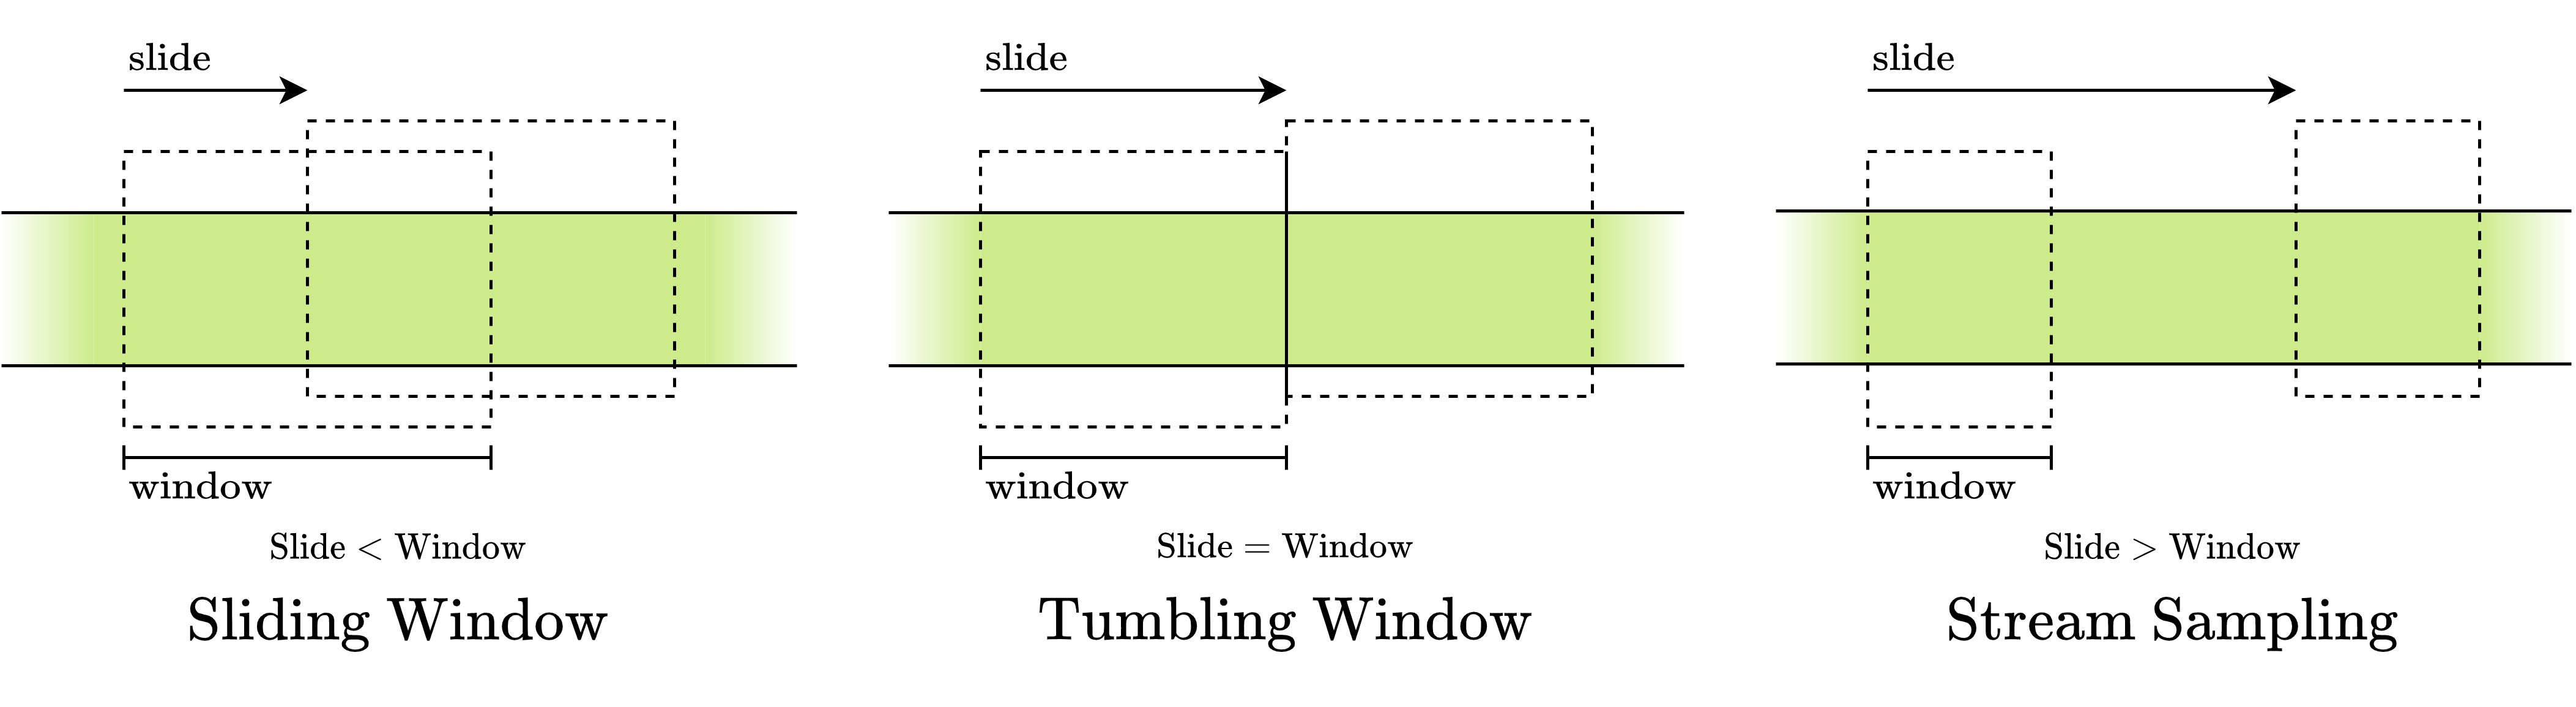
\includegraphics[width=.9\textwidth]{streams/images/window_types.drawio.png}
\end{center}
\textit{Lateness bounds} are an implementation detail for ordering streams
\\ 
\\ \textit{Windows} are SQL supported abstractions for viewing a slice of a stream, and are part of the language semantics.
\begin{sidenotebox}{SQL Windows}
    Despite being originally designed only for persistent databases, SQL added window functions in SQL 2003 (\href{https://en.wikipedia.org/wiki/SQL:2003}{see changelog}).
\end{sidenotebox}
\begin{minted}{sql}
SELECT avg(temp) OVER (
    ORDER BY timestamp
    ROWS BETWEEN 5 PRECEDING AND 5 FOLLOWING
) AS smoothed_temp
FROM SpaceStationTemp;
\end{minted}
We can run aggregate functions on a window:
\begin{minted}{sql}
min, max, sum, count -- Distributive
avg                  -- Algebraic
percentile_cont      -- Holistic
\end{minted}
Percentiles require the entire window to be read (cannot subdivide the window and combine as with \mintinline{sql}{sum}, \mintinline{sql}{count}).
\begin{definitionbox}{Invertible Function}
    \begin{center}
        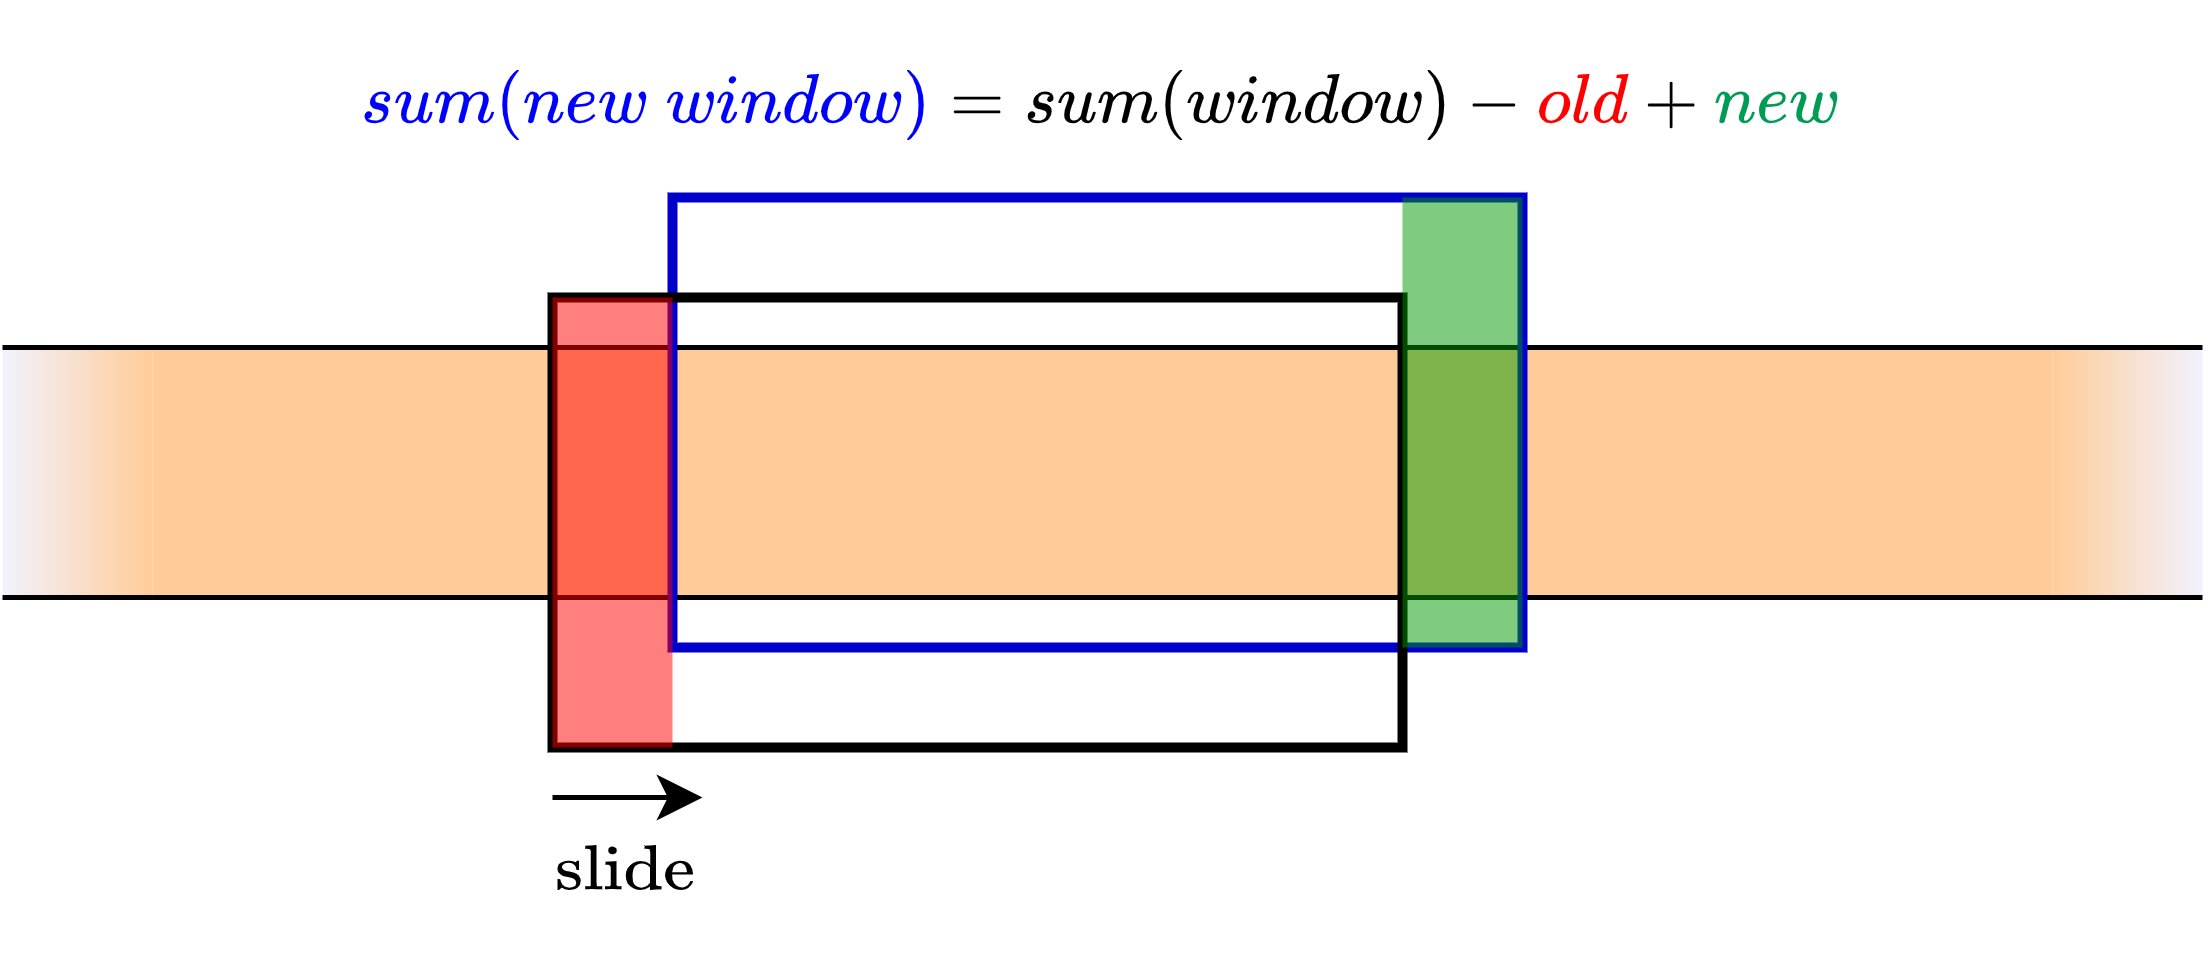
\includegraphics[width=.7\textwidth]{streams/images/invertible_agreggate.drawio.png}
    \end{center}
    Functions with an inverse that can be used to remove rows sliding out of the window from the aggregation.
    \begin{minted}{sql}
sum, count, avg       -- invertible
min, max, percentiles -- non-invertible
    \end{minted}
\end{definitionbox}

\subsection{Aggregate Implementations}
We can implement basic aggregate functions using the previous \mintinline{cpp}{PushOperator<Event>} abstraction.
\subsubsection{Window Sum}
\begin{minted}{cpp}
class WindowSumAggregator : public PushOperator<float> {
    PushOperator<float> *plan_;

    // a circular buffer window
    // the next index after buffer_i_ is the start of the window
    std::vector<float> window_buffer_;

    size_t buffer_i_ = 0;
    float aggregate = 0;

    // for checking the window is filled
    size_t count_ = 0;

public:
    WindowSumAggregator(PushOperator<float> *plan, size_t windowsize) 
      : plan_(plan), window_buffer_(windowsize) {}

    void process(float f) override {
        buffer_i_ = (buffer_i_ + 1) % window_buffer_.size();
        aggregate += f;
        count_++;
        if (count_ > window_buffer_.size()) {
            aggregate -= window_buffer_[buffer_i_];
            window_buffer_[buffer_i_] = f;
            plan_->process(aggregate);
        } else {
            window_buffer_[buffer_i_] = f;
        }
    }
};
\end{minted}

\subsubsection{Window Median}
\begin{sidenotebox}{Improve Me!}
    The provided algorithm must copy the entire window for every \mintinline{cpp}{WindowMedianAggregator::process}. For large window sizes this is very slow, this can be made much more efficient!
\end{sidenotebox}
\begin{minted}{cpp}
class WindowMedianAggregator : public PushOperator<float> {
    PushOperator<float> *plan_;
    std::vector<float> window_buffer_;
    size_t buffer_i_ = 0;

    // for checking the window is filled
    size_t count_ = 0;

public:
    WindowMedianAggregator(PushOperator<float> *plan, size_t window_size) 
      : plan_(plan), window_buffer_(window_size) {}

    void process(float f) override {
        const size_t size = window_buffer_.size();
        buffer_i_ = (buffer_i_ + 1) % size;
        window_buffer_[buffer_i_] = f;
        count_++;
        if (count_ > size) {

            // copy and sort, this can be made much more efficient using a multiset and vector
            // see multiset median trick: https://codeforces.com/blog/entry/68300
            std::vector<float> sorted = window_buffer_;
            std::sort(sorted.begin(), sorted.end());

            // if even size get average of two middle, else middle element
            if (size % 2 == 0) {
                plan_->process((sorted[size / 2] + sorted[(size / 2) - 1]) / 2);
            } else {
                plan_->process(sorted[size / 2]);
            }
        }
    }
};
\end{minted}


\subsection{Two Stacks Algorithm}
\begin{center}
    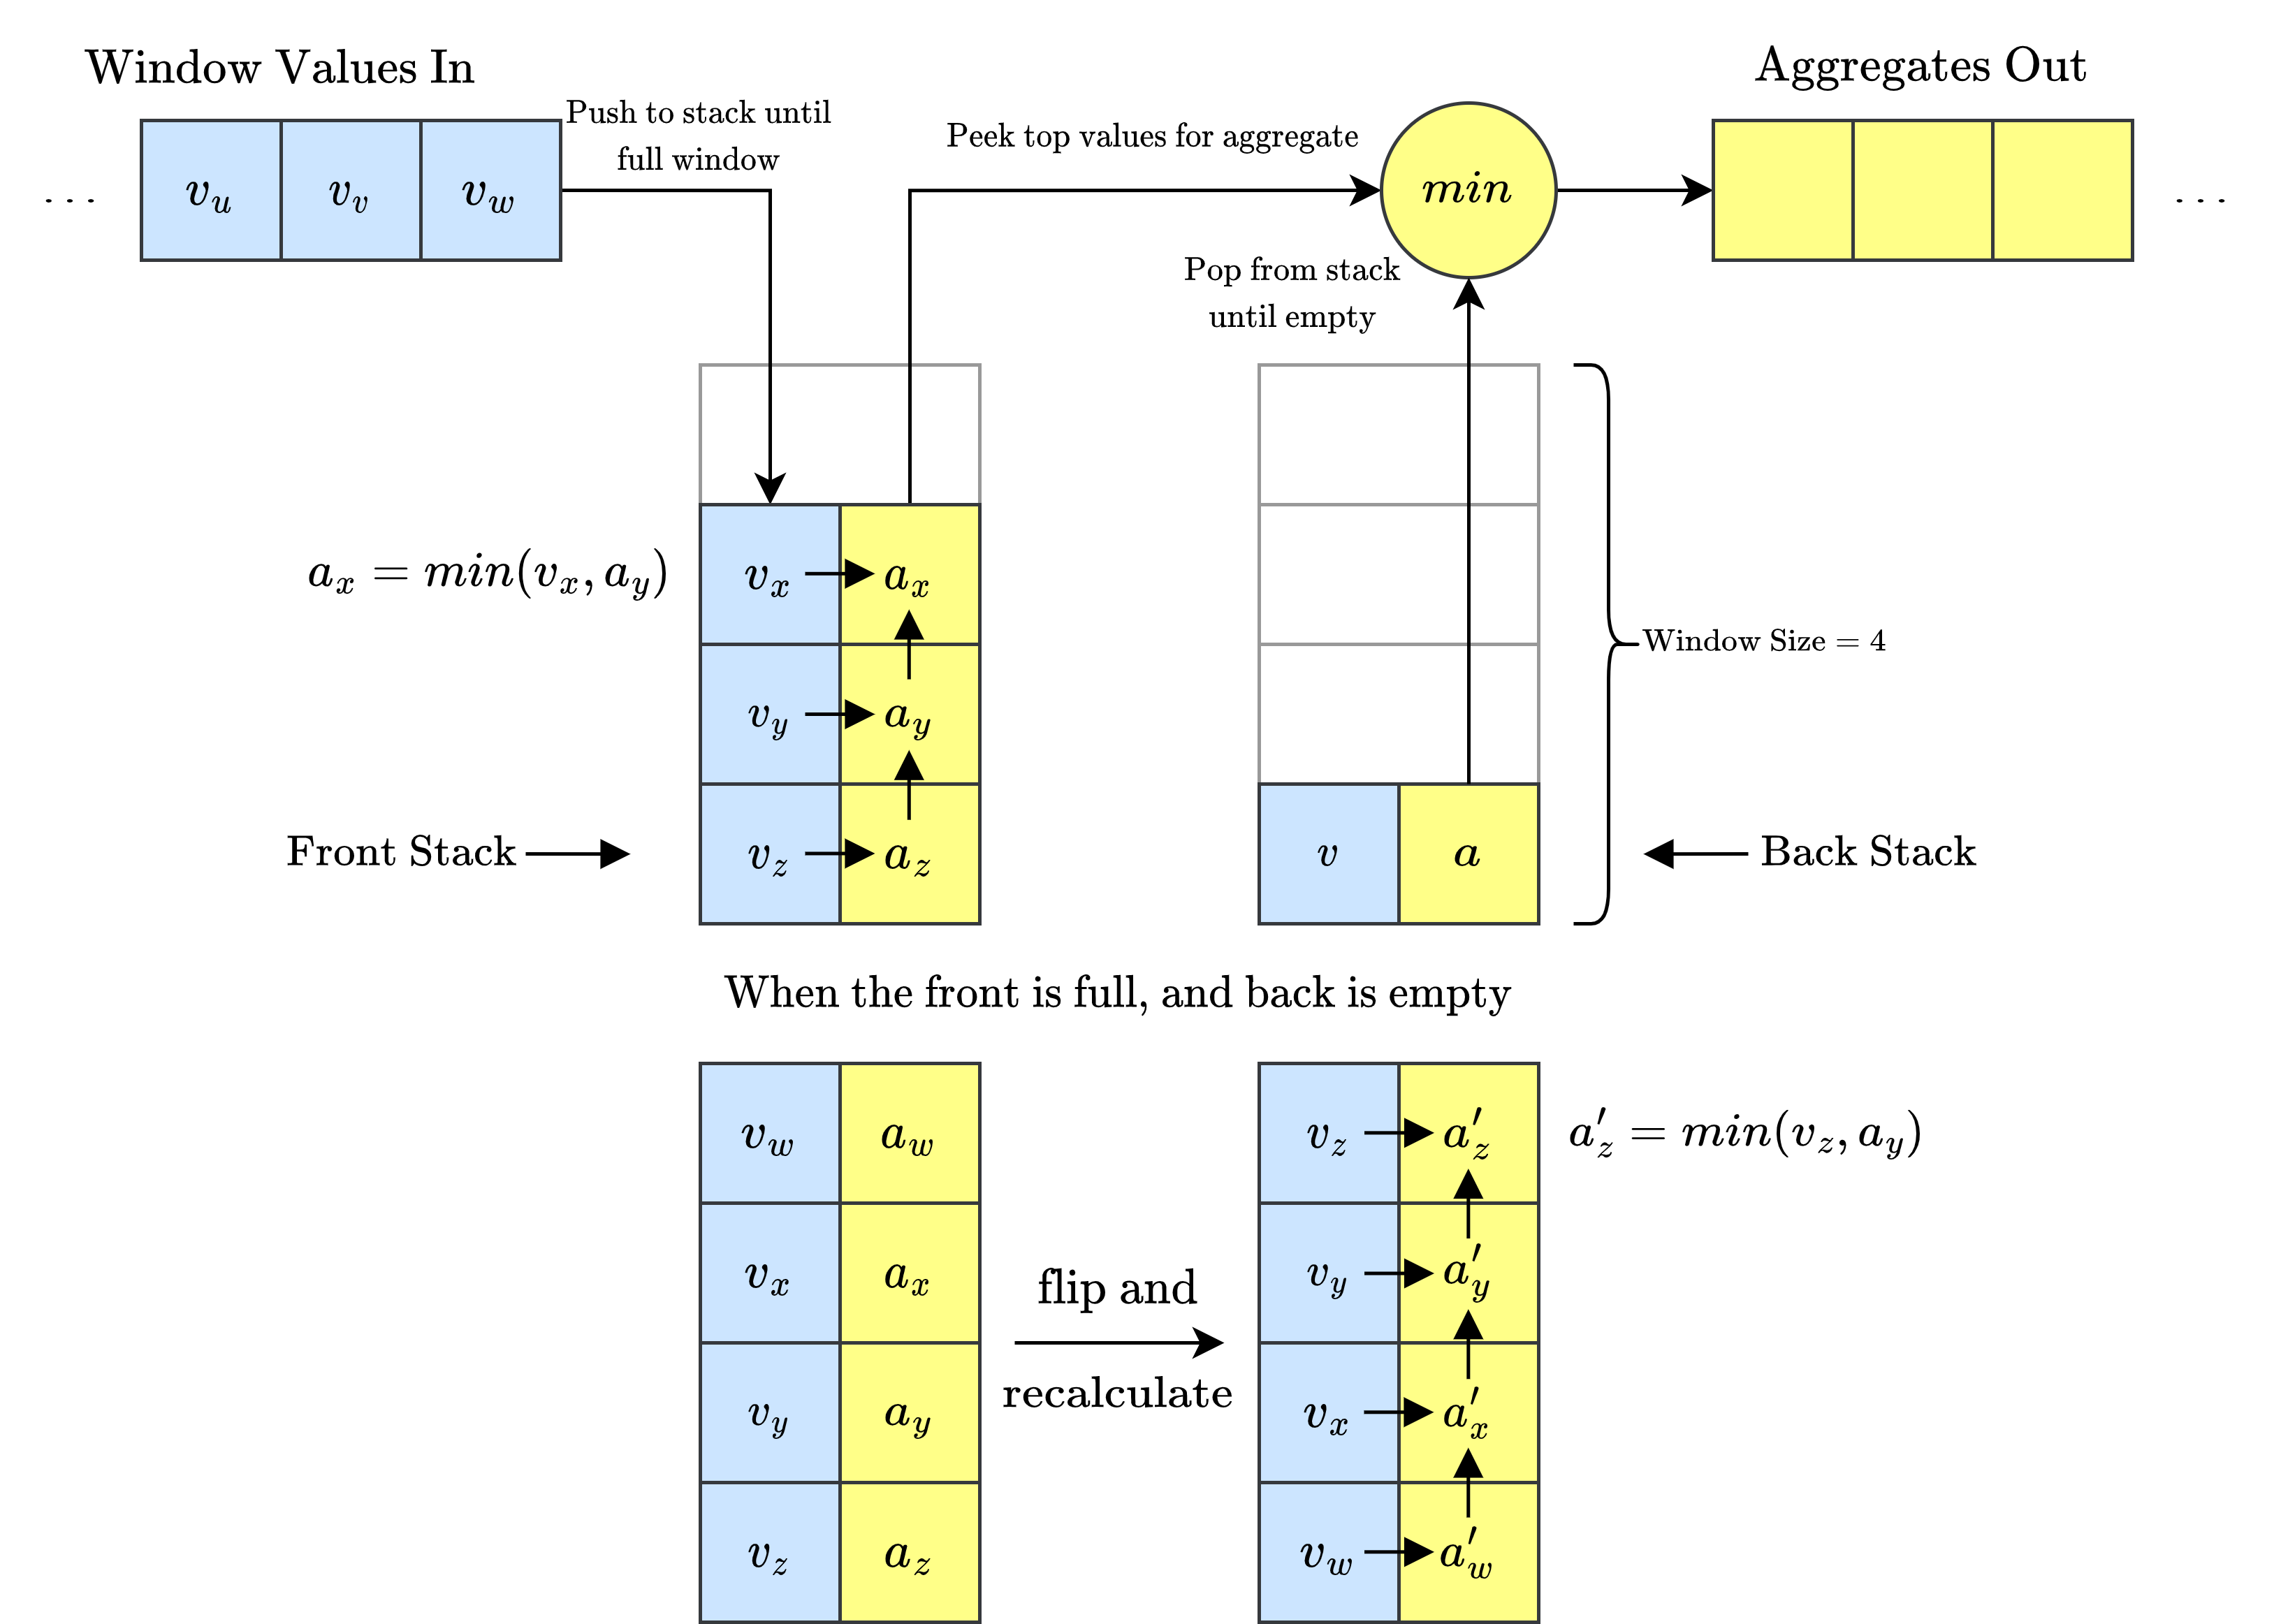
\includegraphics[width=.9\textwidth]{streams/images/two_stacks.drawio.png}
\end{center}
Two stacks of max size $window \ size$ are kept.
\begin{itemize}
    \item Each contains aggregates calculated from below adjacent aggregates and current value.
    \item When the front stack is full, and back stack empty (occurs every $\cfrac{1}{window \ size}$) flip the front stack, recalculate aggregates and set to back stack.
\end{itemize}
We can implement this using the previous \mintinline{cpp}{PushOperator<Event>} abstraction.
\begin{minted}{cpp}
template <typename Event, Event agg(Event &, Event &)>
class WindowTwoStackAggregator : public PushOperator<Event> {
    PushOperator<Event> *plan_;

    // front stack
    std::vector<Event> front_values_;
    std::vector<Event> front_agg_;

    // back stack
    std::vector<Event> back_values_;
    std::vector<Event> back_agg_;

    // track the top of front and back stacks
    size_t window_pos = 0;

    // to determine when to start outputting aggregates
    size_t count_ = 0;

    // flip front stack to back stack, sets window_pos = 0
    // invariant: Must have window_size items present
    void flip() {
        size_t size = front_values_.size();
        assert(window_pos == size);

        for (size_t i = 0; i < size; i++) { back_values_[size - 1 - i] = front_values_[i]; }

        back_agg_[0] = back_values_[0];

        for (size_t i = 1; i < size; i++) { back_agg_[i] = agg(back_agg_[i - 1], back_values_[i]); }

        window_pos = 0;
    }

    // Push an item to the front_stack, leaves the window_pos untouched
    void push_front(Event r) {
        if (window_pos == 0) {
            front_values_[0] = r;
            front_agg_[0] = r;
        } else {
            front_values_[window_pos] = r;
            front_agg_[window_pos] = agg(r, front_agg_[window_pos - 1]);
        }
    }

public:
    WindowTwoStackAggregator(PushOperator<Event> *plan, size_t window_size) 
      : plan_(plan), front_values_(window_size), front_agg_(window_size), 
        back_values_(window_size), back_agg_(window_size) {}

    void process(Event r) override {
        size_t max_size = front_values_.size();
        if (count_ < max_size) {
            push_front(r);
            window_pos++;
        } else {
            if (window_pos == max_size) { flip(); }

            push_front(r);
            plan_->process(agg(front_agg_[window_pos], back_agg_[max_size - 1 - window_pos]));
            window_pos++;
        }
        count_++;
    }
};
\end{minted}
For example:
\begin{minted}{cpp}
Output<int> console(std::cout);
WindowTwoStackAggregator<int, intmax> maxints(&console, 3);
UserInput<int> user(&maxints, std::cin);
user.run();
\end{minted}
\begin{minted}{Bash}
1
2
3
->3
1
->3
1
->3
1
->3
1
->1
5
->5
4
->5
\end{minted}

\section{Stream Joins}
\subsection{Handshake Join}
\begin{definitionbox}{Handshake Join}
    \begin{center}
        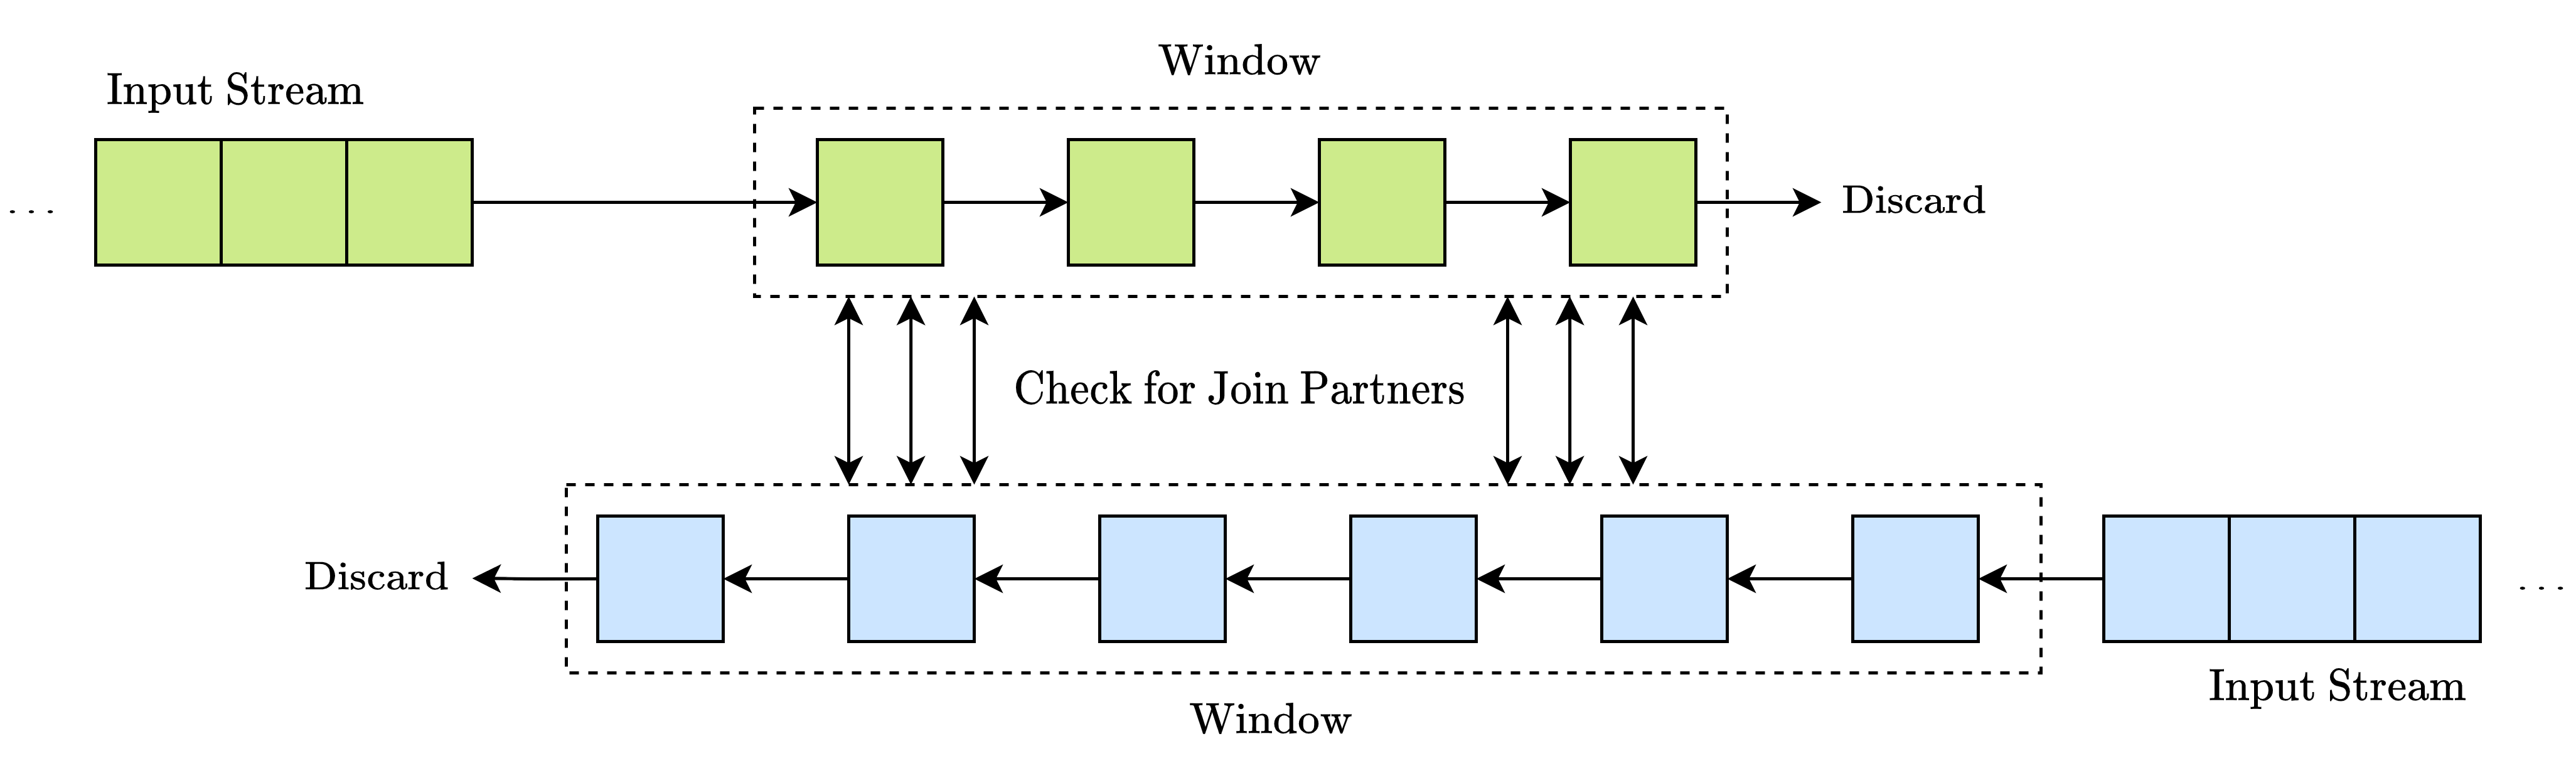
\includegraphics[width=\textwidth]{streams/images/handshake_join.drawio.png}
    \end{center}
    \begin{itemize}
        \item A \textit{nested loop join} joining over a window.
        \item Can be optimised for parallel window joins.
        \item Only works for window queries.
    \end{itemize}
\end{definitionbox}

\subsection{Symmetric Hash-Joins}
\begin{definitionbox}{Symmetric Hash-Joins}
    \begin{center}
        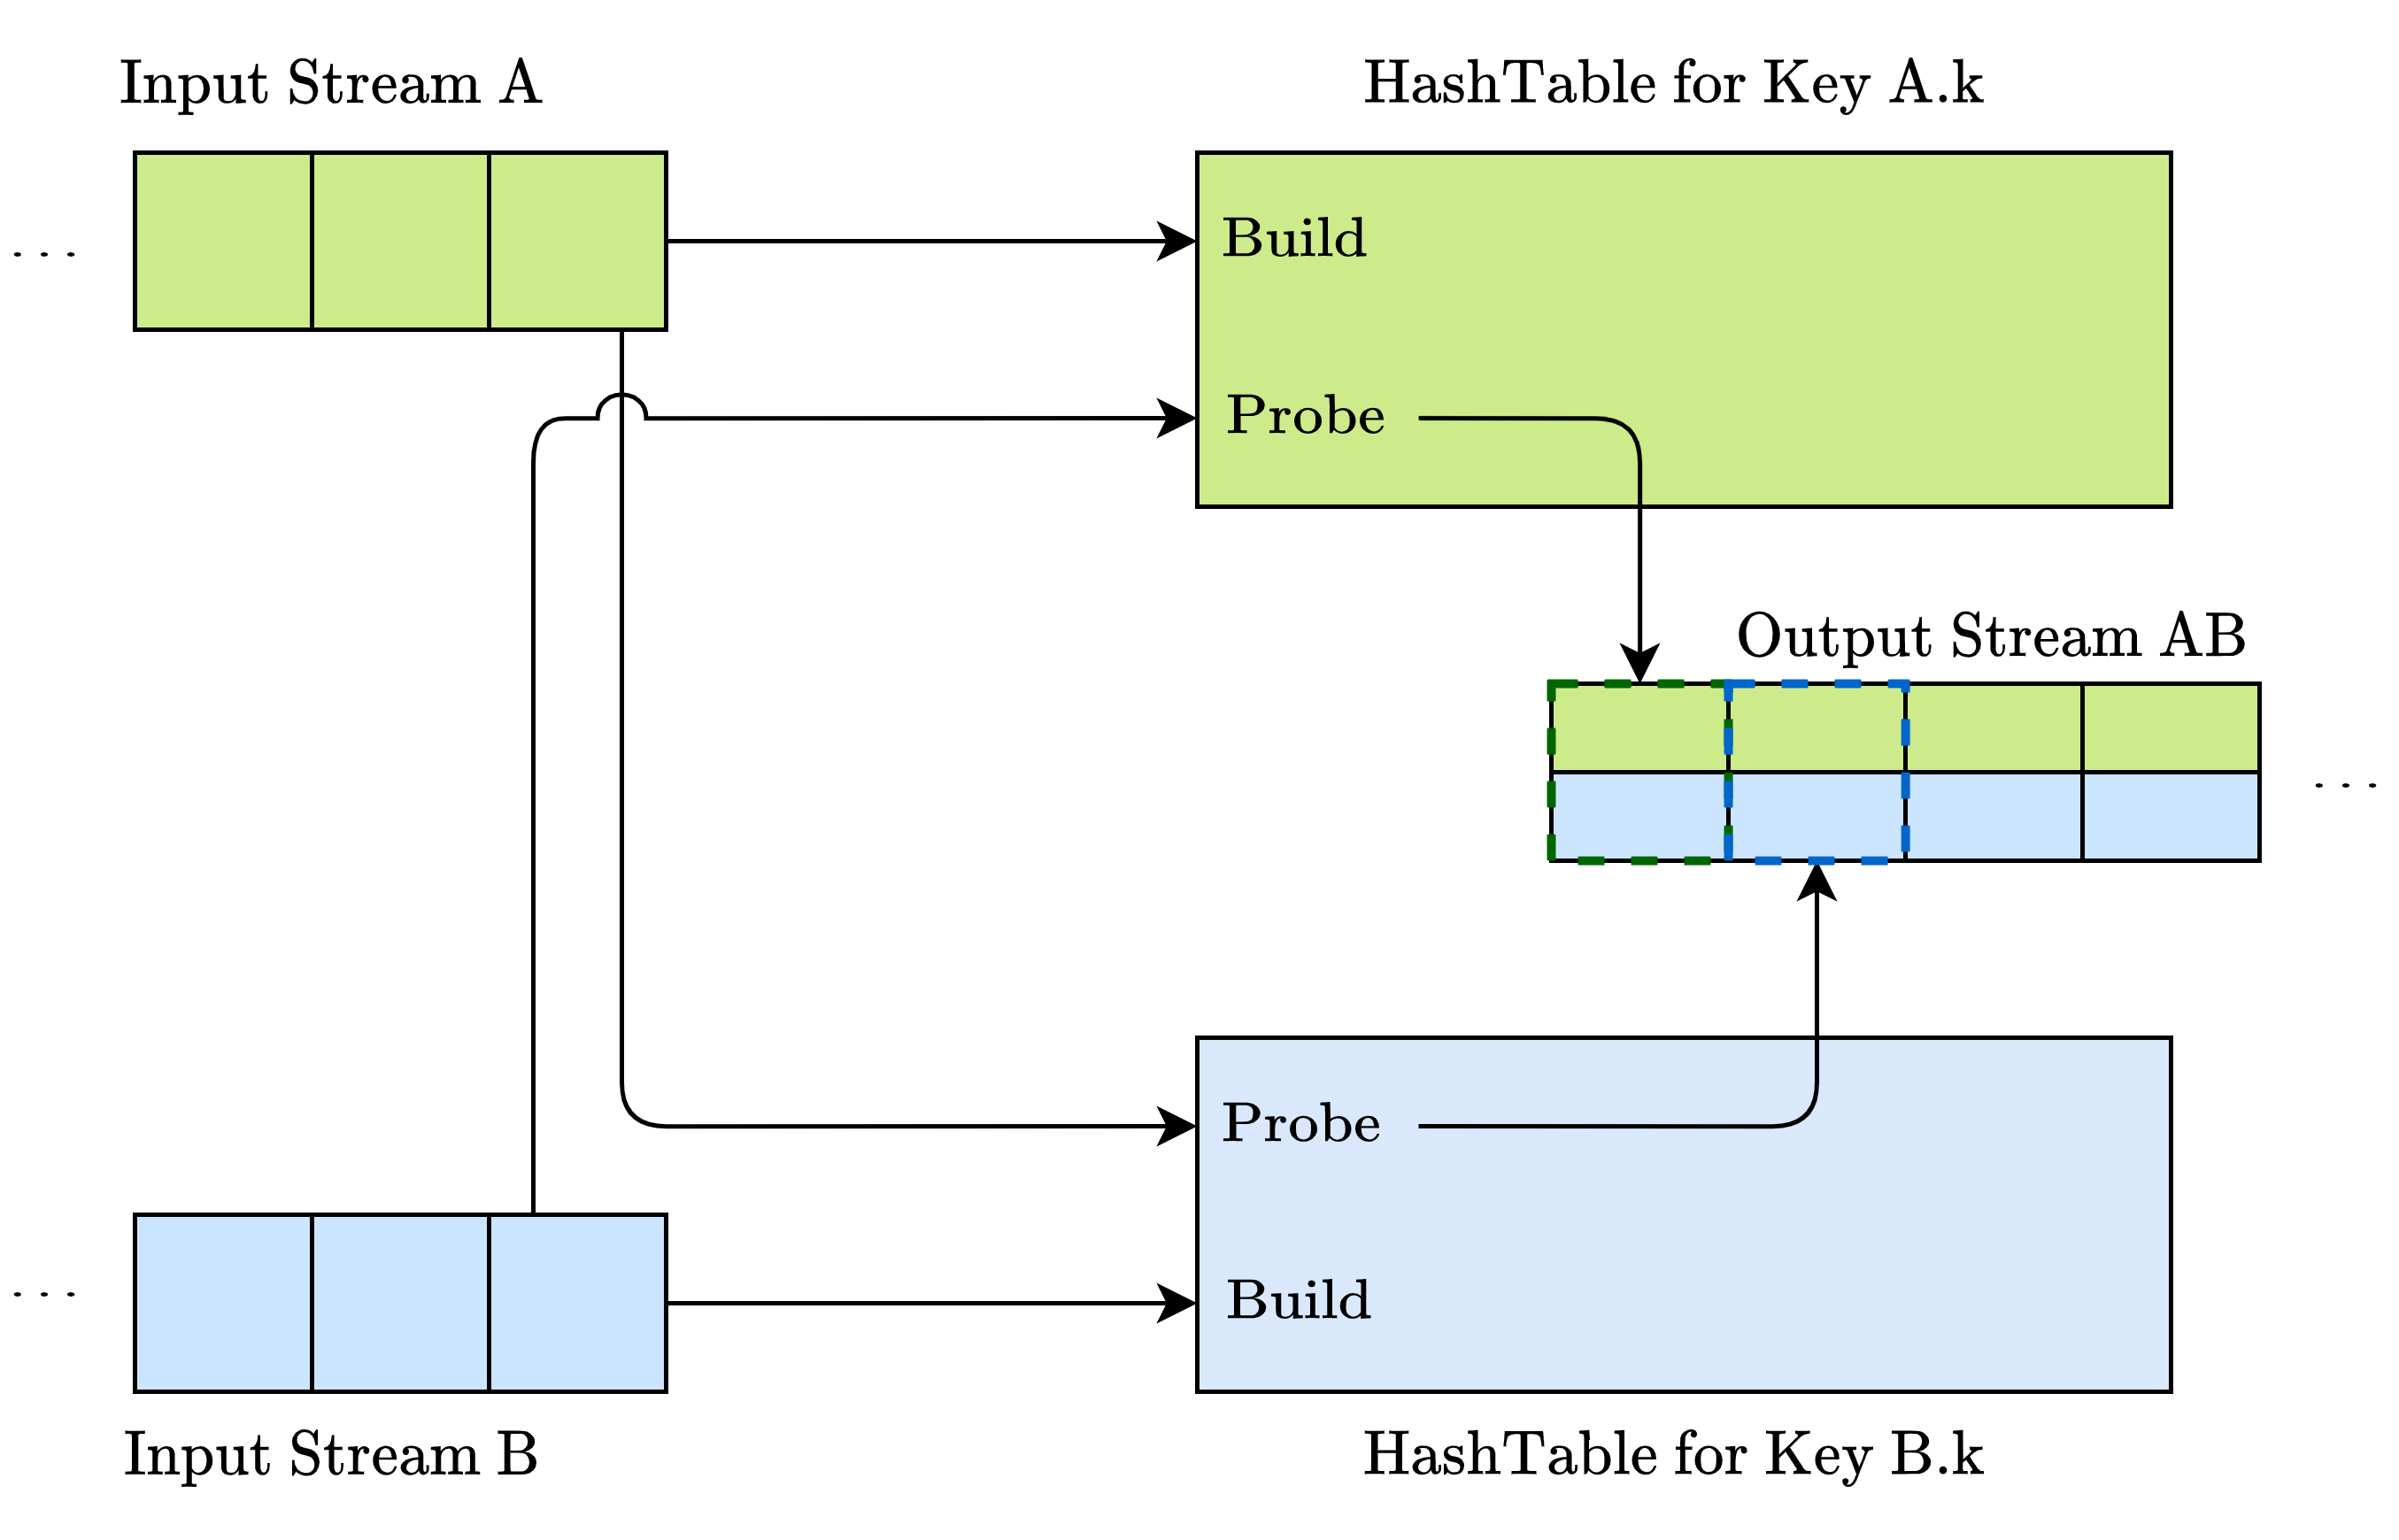
\includegraphics[width=.7\textwidth]{streams/images/symmetric_hash_join.drawio.png}
    \end{center}
    Both input streams build their own hashtable, while probing the other. Matches from probes are inserted into the joined output stream.
    \begin{itemize}
        \item A \textit{pipelineable} hash join
        \item Does not have a equivalent window oriented version
        \item Hashtables grow with unbounded input streams, so needs some form of garbage collection of older / not joinable hashtable entries.
    \end{itemize}
\end{definitionbox}

\subsection{Bloom Filters}
\begin{definitionbox}{Bloom Filter}
    \begin{center}
        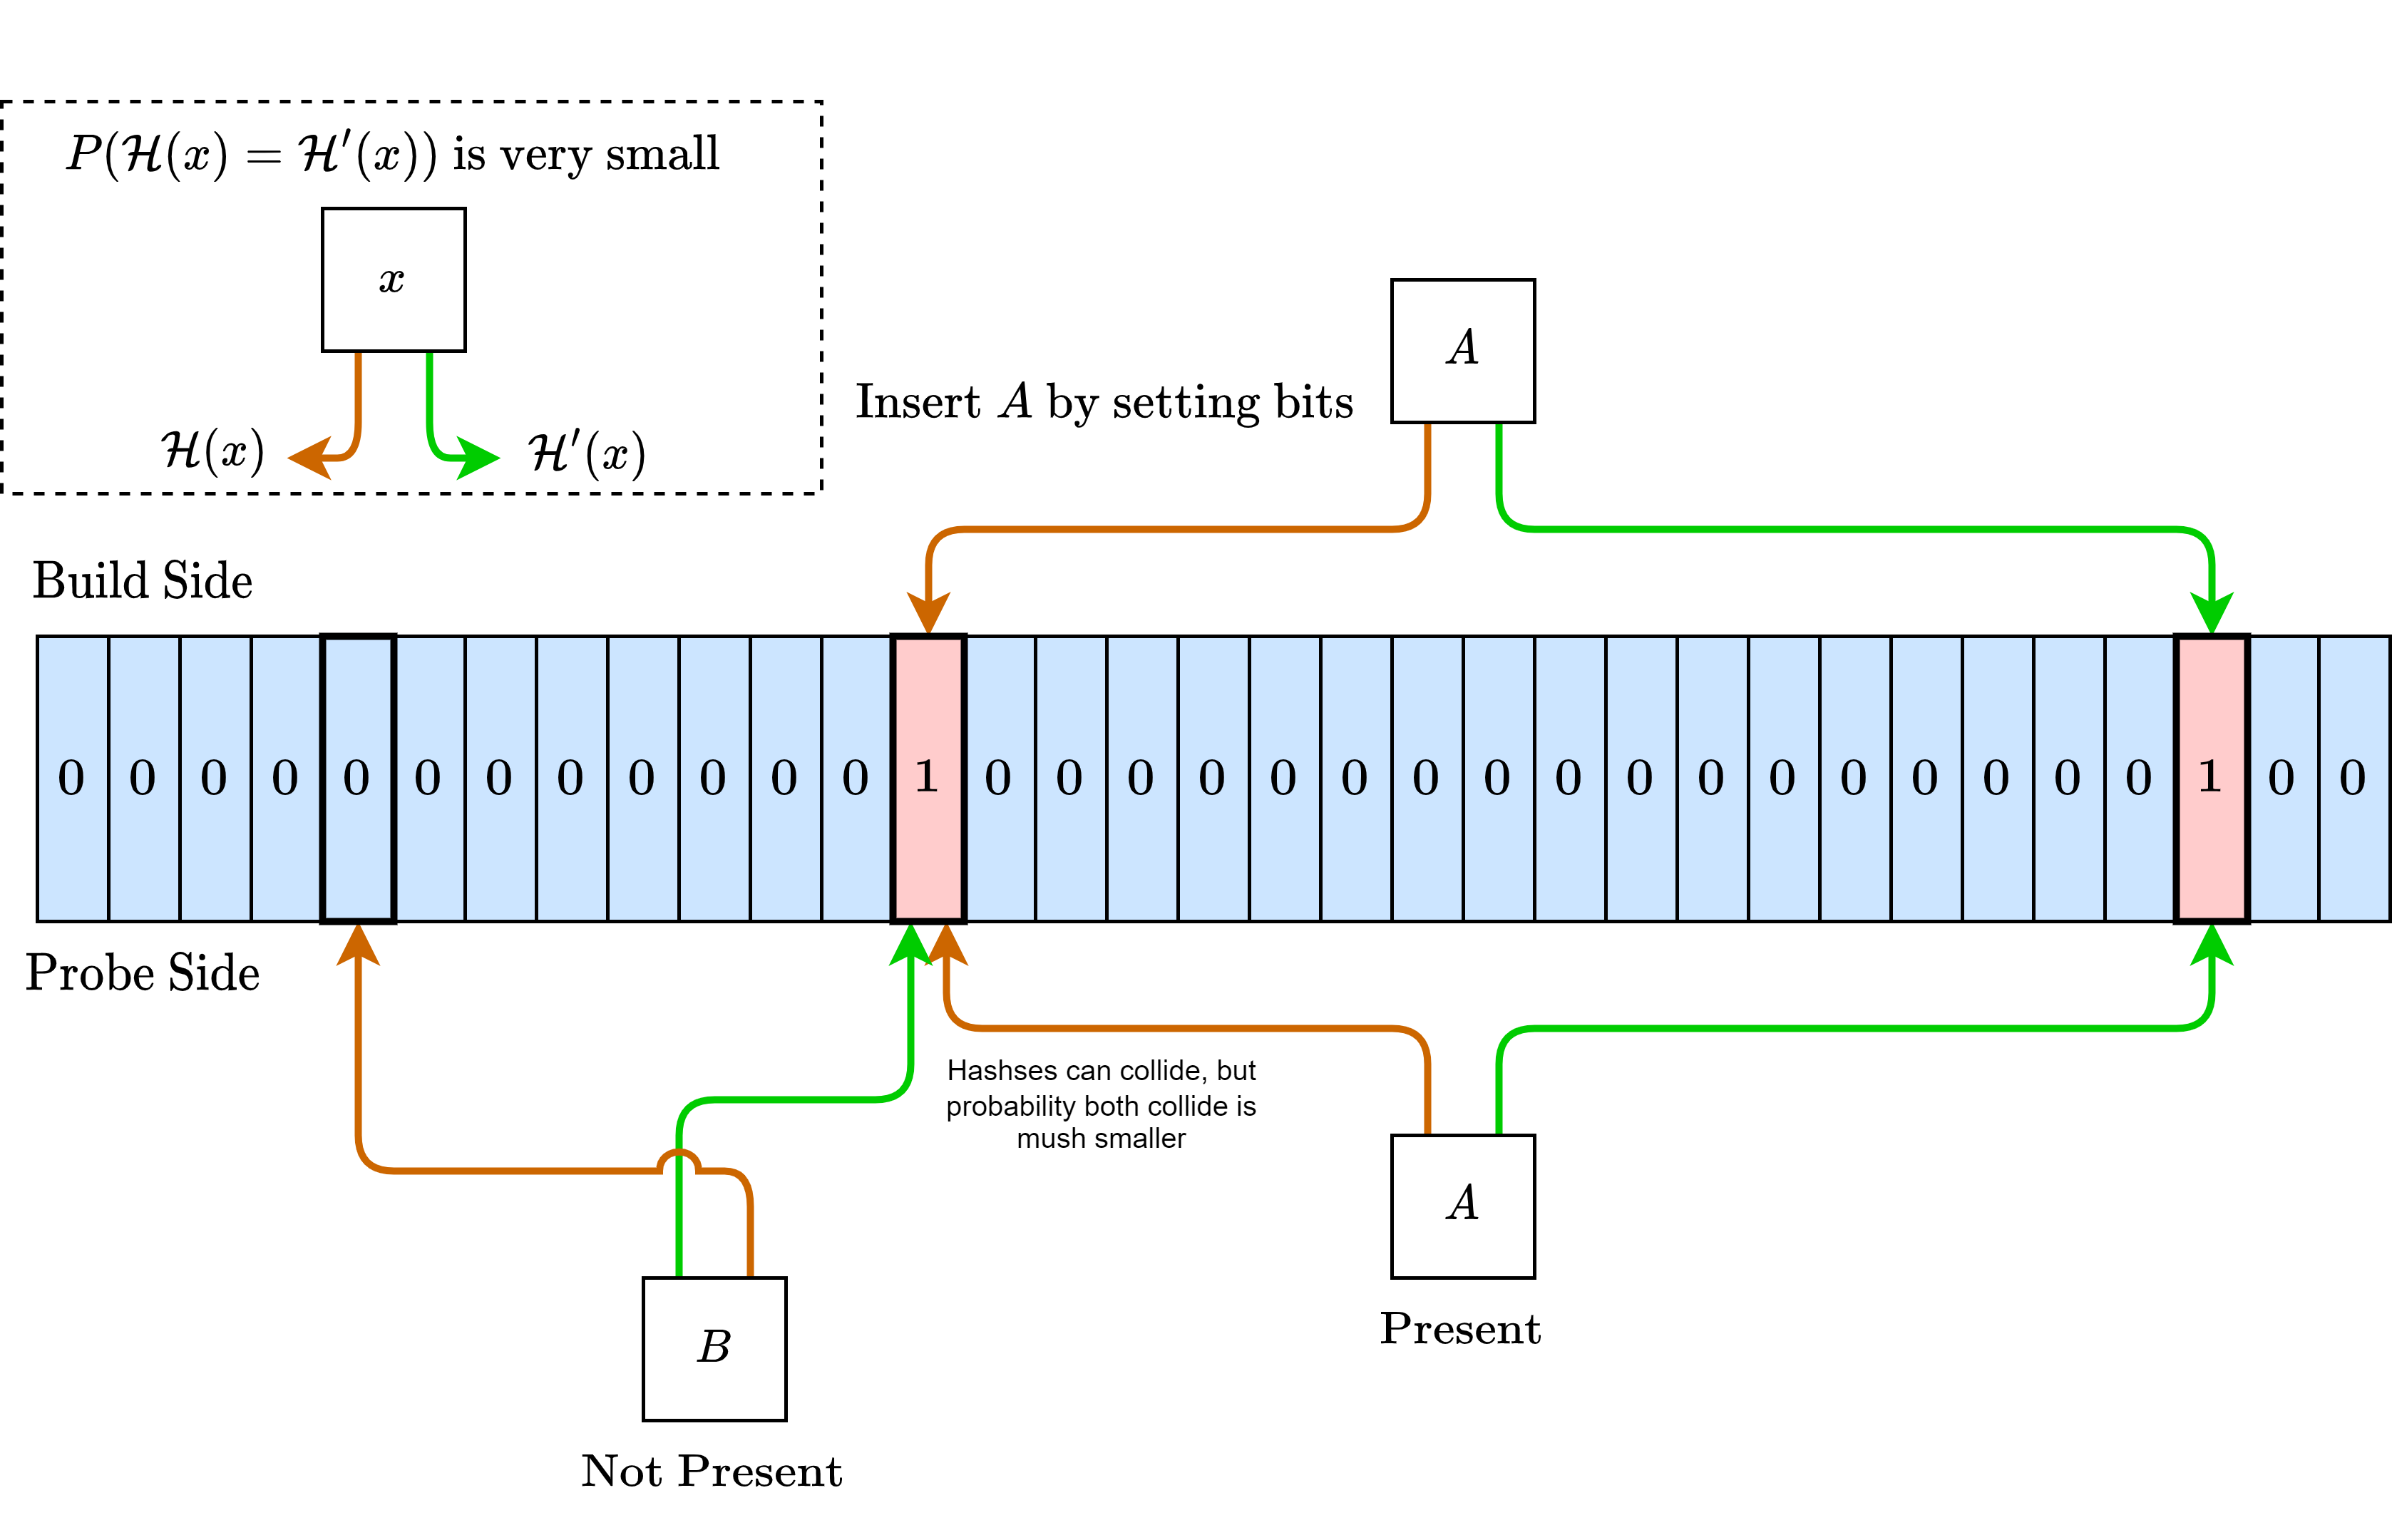
\includegraphics[width=\textwidth]{streams/images/bloom_filter.drawio.png}
    \end{center}
    A table of bits, indexed by hashing the key used for the join. By using multiple independent hashes, the probability all collide is low.
    \begin{itemize}
        \item Collisions/false-positives still possible.
        \item Can use as many independent hashes as needed.
        \item Uses finite space.
        \item Can be used to implement a form of symmetric hash-join.
    \end{itemize}
\end{definitionbox}
\subsubsection{Tuning Bloom Filters}
\noindent Bloom filters have several parameters that can be tuned.
\\ \begin{tabular}{l p{.7\textwidth}}
    $m$        & bits in filter \\ 
    $n$        & expected number of distinct elements \\ 
    $k$        & number of hash functions \\ 
    $\epsilon$ & False-positive rate \\
\end{tabular}
\[\begin{matrix}
    m \cong -1.44 \times n \times \log_2(\epsilon) & \ &
    k \cong \cfrac{m}{n} \times \log_e(2) & \ &
    \epsilon  = \left( 1 - e^{-\cfrac{k \times n}{m}}\right)^k \\
\end{matrix}\]
